state estimation to be designed will be deployed in two cars
non-autonomous EV, newly built -> sensors can be chosen
partly autonomous DV, reuse old car with camera/lidar -> fixed set of sensors

\section{Vehicle Characteristics}
car is equipped with a plethora of sensors, but only some are important to us
e.g., sensors for brake pressure or accelerator pedal actuation not relevant
top down view of car with sensor positions
table: sensor name, sensor type, measured variables, columns EV and dv with X
refer to characterization in TC paper
sfii is key sensor for velocity estimation because it is slip free as opposed to wheels and fast as opposed to GPS
 (compare velocity with only gps, sfii and whee)

ES910 as ECU, can be programmed in Matlab/Simulink, C, ASCET-MD~\cite[p.~17]{ETASGmbHStuttgart.2018}
runs \gls{vdc} with TC, TV, motor request...
The VDC is a tool that helps the driver to exploit the maximum physical potential of the vehicle.
state estimation will be part of \gls{vdc}
In DV vehicle, DV software runs on a separate computer that needs part of state as well
inputs from sensor via CAN at different frequencies to avoid congestion
it is unclear whether sfii will be in DV

\section{Requirements}
goal: provide robust, accurate estimate of vehicle state for \gls{vdc} and DV software 
flexible: support arbitrary sensor setups within full sensor setup
robust: detect and handle sensor failures
state variables to estimate
estimate these variables in CoG, this describes motion of vehicle since it is assumed to be a rigid body
real-time: needs to be computable in 1 ms frequency
complete in all areas, so no developments in near future are necessary

design principle: use simple methods if they work just as well (occam's razor)
only if the results are not adequate, try more complicated approaches
easier to understand and troubleshoot
make less assumptions and thus generalize better
because maintainers change every year
on a higher level, clear architecture to facilitate maintenance and extension

We assume that vertical dynamics are negligible and only motion in the two-dimensional plane of the track are relevant, simplifying equations.

\section{Architecture}
in the literature, there is no concrete solution for our problem
however, we can combine common components into our own solution

At high level: state estimation = preprocessing + outlier detection + state estimation
To fulfill requirements of robustness and accuracy: outlier detection and sensor fusion
For practical reasons: preprocessing
preprocessing and outlier detection for each sensor in parallel
all IMUs have same treatment
out bus creation calculates vehicle side slip angle from vx and vy

For flexibility: outlier detection and sensor setup detection using same mechanism
in both cases, sensor cannot or should not be used in sensor fusion
does not matter if not connected, not sending, invalid values

\begin{figure}[h]
	\centering
	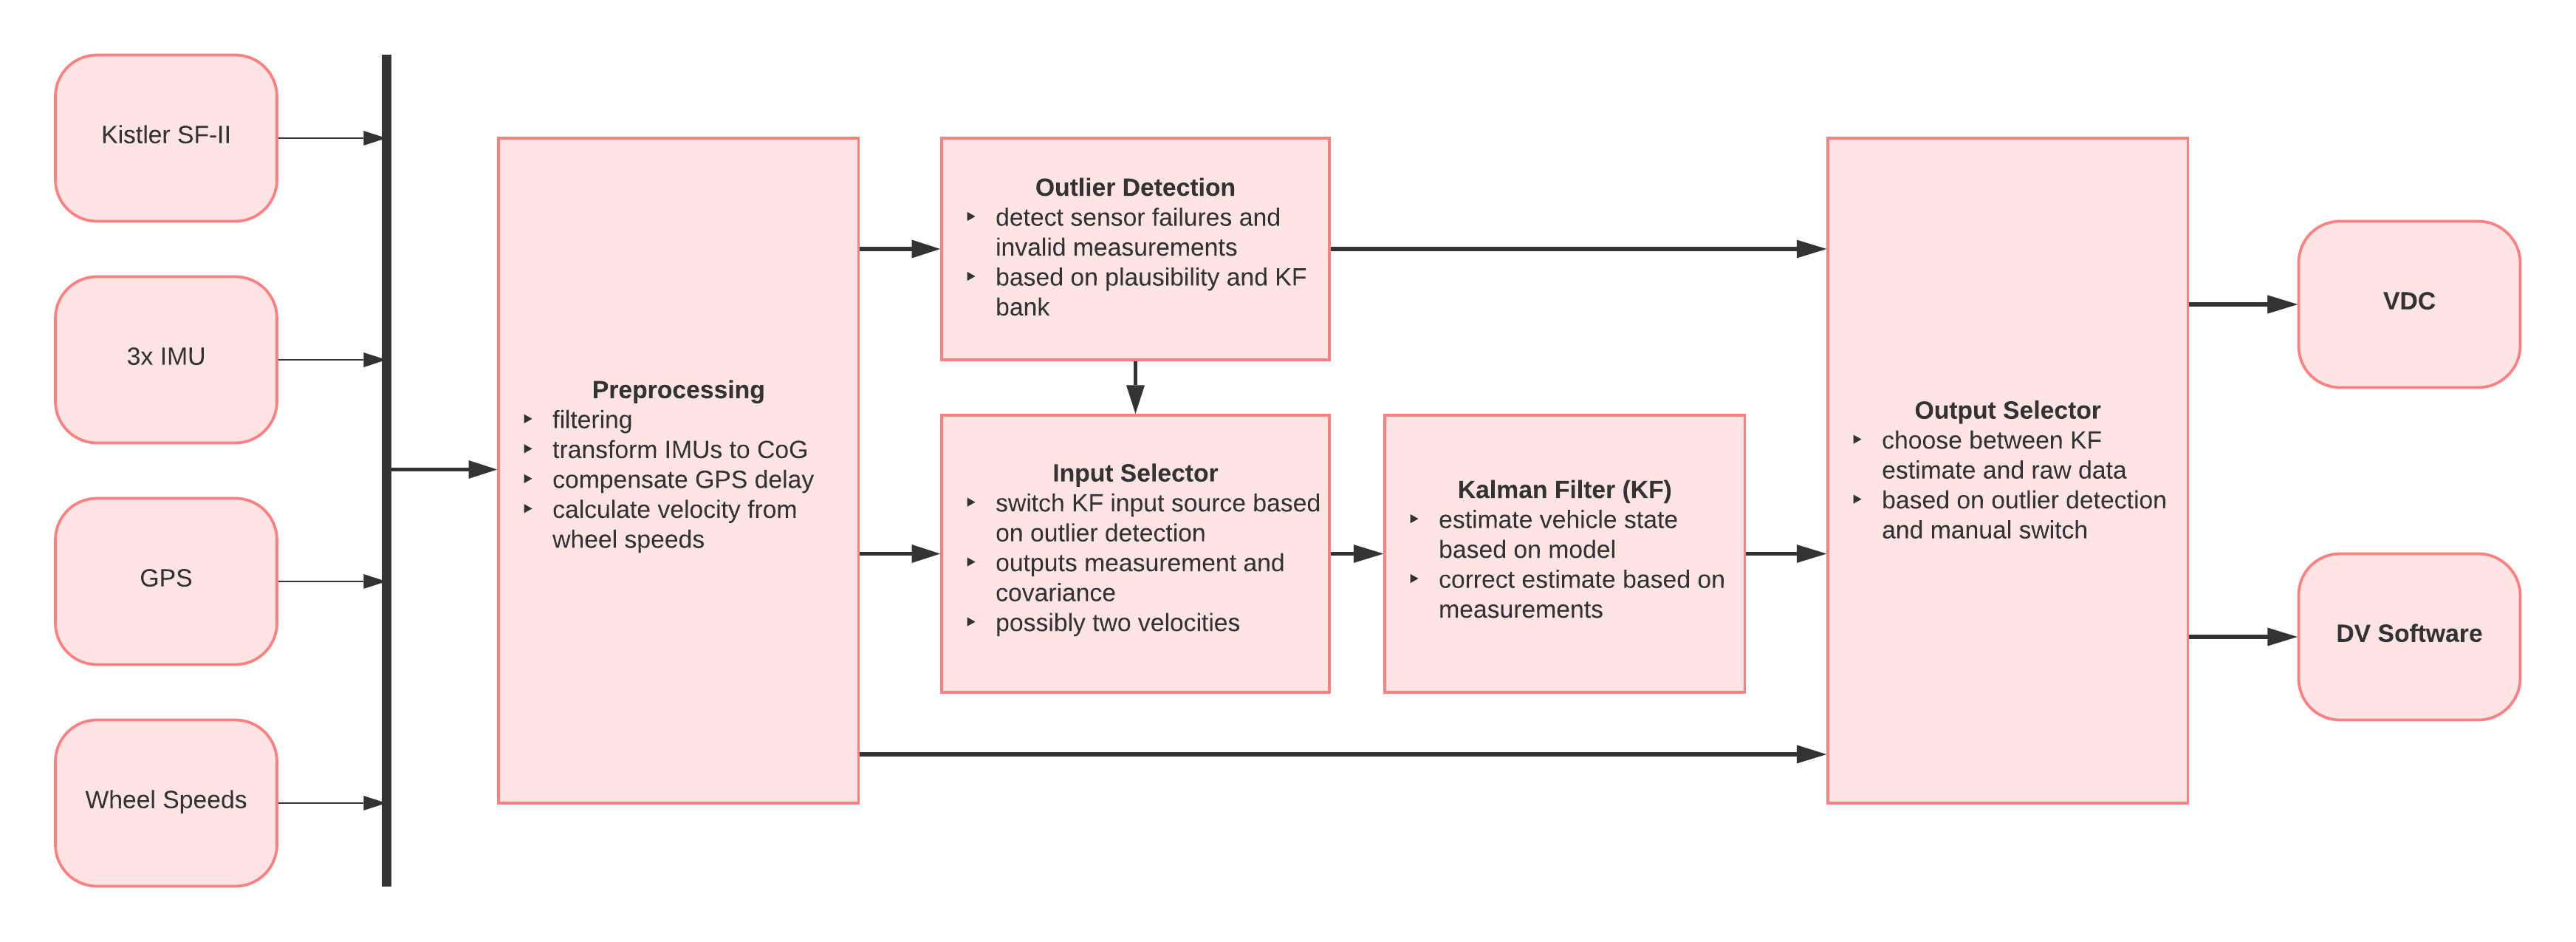
\includegraphics[width=\textwidth]{architecture}%
	\caption{High-level architecture}
	\label{fig:architecture}
\end{figure}
Show all inputs and outputs

\section{Preprocessing}
convert to SI units and deg to rad so formulas can be applied
show necessary transformations for each measurement

IMU fusion
very important because used extensively in EKF and other parts of VDC like TC and TV (especially dpsi)
fast response
contains outlier detection because available sensors need to be known before fusion in preprocessing

GPS WGS84 coordinates transformed to track with first known point as origin

sfii transformed to \gls{cog}

\section{Outlier Detection}
Show diagram of AND and OR
For all EKF inputs
Plausibility check for all
For velocity, use wheels, GPS and sfii in EKF bank, different covs than in normal EKF
Plausibility for velocities rather conservative
observability and controllability
goal: support one sensor failure, more is unlikely

debouncing to increase robustness
allow manual three-way override to enable/disable sensors and override outlier detection errors

\section{EKF}
outlier detection sensor state is used to create measurement mask
Show input selection and state equations, jacobians
euler forward discretization
GPS is not included because it is not beneficial due to its slow response
kinematic model from~\cite[p.~156]{AlexanderWischnewski.2019}


prediction using differential equation
initialization
disable measurements using separate mask
input cov as process noise
